\documentclass[letterpaper,11pt]{article}
\usepackage{graphicx}
\usepackage{listings}
%\usepackage{datetime}

\lstset{
	breaklines=true
}

\begin{document}

\begin{titlepage}

\begin{center}

\Huge{Assignment 1}

\Large{CS 595:  Introduction to Web Science}

\Large{Fall 2013}

\Large{Shawn M. Jones}

\Large Finished on \today

\end{center}

\end{titlepage}

\newpage
\section*{1}

\subsection*{Question}

\begin{verbatim}
Demonstrate that you know how to use "curl" well enough to
correctly POST data to a form.  Show that the HTML response that
is returned is "correct" (e.g., save it to a file and then view
that file in a browser and take a screen shot).
\end{verbatim}

\subsection*{Answer}

The \verb+curl+ command can be used to post data to a form in several ways, but the most easy is the following:
\begin{lstlisting}[frame=single]
curl --data 'variable1=value1&variable2=value2' \
  http://www.example.com
\end{lstlisting}

The more difficult prospect is finding a URI on the Internet that accepts form submission without authentication.  Fortunately, my recent work in using Mediawiki has led me to a web application that accepts formatted CSV and returns a table formatted in Mediawiki syntax.

I posted the CSV data ``1,2'' to the form like so:
\begin{lstlisting}[frame=single]
curl -i --data 'csv=1,2&separator=,&quotes=&quot;&escape=\&break=SPACE&convert=html&output_encoding=UTF-8&to_wp=Convert+To+Mediawiki!'
   http://area23.brightbyte.de/csv2wp.php
\end{lstlisting}

and got back the following response from \verb+curl+:
\begin{lstlisting}[frame=single]
HTTP/1.1 200 OK
Date: Sat, 31 Aug 2013 23:20:02 GMT
Server: Apache/2.2.16 (Debian)
X-Powered-By: PHP/5.3.3-7+squeeze16
Content-Description: csv2wp-1377991202.UTF-8.txt
Content-Length: 23
Content-Type: text/plain; charset=UTF-8

{|
|1
|2
|----
|}
\end{lstlisting}

Executing again, without -i, saves the data to a file:
\begin{lstlisting}[frame=single]
curl --data 'csv=1,2&separator=,&quotes=&quot;&escape=\&break=SPACE&convert=html&output_encoding=UTF-8&to_wp=Convert+To+Mediawiki!'
   http://area23.brightbyte.de/csv2wp.php \
   > work/q1out.txt
\end{lstlisting}


which renders in the browser like shown in Figure {\ref{fig:q1screenie}.

\begin{figure}
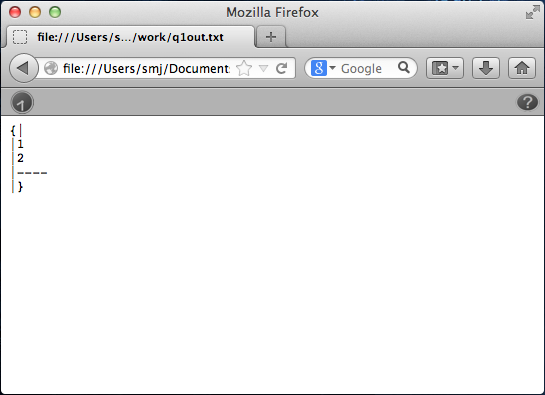
\includegraphics[scale=0.7]{work/q1screenie.png}
\caption{The output of the curl command, rendered in Mozilla Firefox}
\label{fig:q1screenie}
\end{figure}




\newpage
\section*{2}

\subsection*{Question}

\begin{verbatim}
Write a Python program that:
1. takes one argument, like "Old Dominion" or "Virginia Tech"
2. takes another argument specified in seconds (e.g., "60" for 
   one minute).
3. takes a URI as a third argument: 
   http://sports.yahoo.com/ncaa/football/scoreboard
   or
   http://sports.yahoo.com/ncaa/football/scoreboard?w=1&c=all&y=2012
   or
   http://sports.yahoo.com/ncaa/football/scoreboard?w=2&c=all&y=2012
   etc.
4. downloads the URI, finds the game corresponding to the team
   argument, prints out the current score (e.g., "Old Dominion 27, 
   East Carolina 17), sleeps for the specified seconds, and then
   repeats (until control-C is hit).
\end{verbatim}

\subsection*{Answer}

\lstinputlisting[language=Python,frame=single]{work/gimmescore.py}

\newpage
\section*{3}

\subsection*{Question}

\begin{verbatim}
Consider the "bow-tie" graph in the Broder et al. paper (fig 9):
http://www9.org/w9cdrom/160/160.html

Now consider the following graph:

A --> B
B --> C
C --> D
C --> A
C --> G
E --> F
G --> C
G --> H
I --> H
I --> J
I --> K
J --> D 
L --> D
M --> A
M --> N
N --> D
    
For the above graph, give the values for:

IN: 
SCC: 
OUT: 
Tendrils: 
Tubes: 
Disconnected:
\end{verbatim}

\subsection*{Answer}
The following is a graph of the included points, generated using Graphviz.
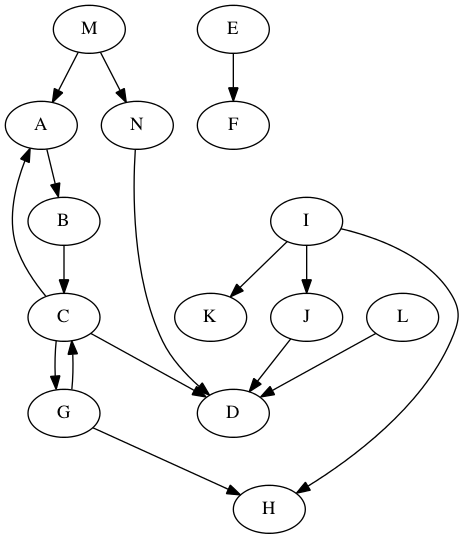
\includegraphics[scale=0.5]{work/q3.png}

The descriptions of each node is a matter of interpretation.  Explanations have been provided for each value assignment.

\textbf{IN:}  $M$

The IN components form the starting point for connection to the SCC.  They all sit at the start of the graph.  In this graph, because of how the SCC and tubes are defined, the only IN component is $M$.

\textbf{SCC:}  $A, B, C, G$

The Strongly Connected Component consists of those heavily linked items connected to from the list of nodes listed as part of IN.  It's an $A, B, C, G$ world.

\textbf{OUT:}  $D$

The only member of OUT is $D$, who forms a sink from members of the SCC and the tendrils.

\textbf{Tendrils:}  $I, J, K, L$

The tendrils come from other graphs and only join the whole via $D$.

\textbf{Tubes:} $N$

$N$ is a tube linking from $M$ (from IN) to $D$ (from OUT).

\textbf{Disconnected:}  $E, F$

The Disconnected components link to no one in the graph, and stand alone.

Note that other interpretations are possible.  For example, the SCC could consist of $A, B, C, D, G, J, N$ with IN containing $M, I, L$ and with no OUT.  In that case, there's no real tube ($H$ is a sink, so it's not really linking \emph{around} the SCC), because there's no OUT to connect to, and there are no tendrils.

\end{document}